\section{Chapter 3: Lightness, Brightness, Contrast and Constancy}
\graphicspath{ {pngs/ch3/} }
%    \begin{figure}[H]
%        \centering
%        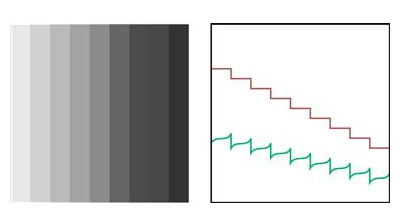
\includegraphics[width=0.4\textwidth]{chevreul_illusion.png}
%        \caption{Chevreul illusion, grayscale step patterns}
%    \end{figure}



\secttoc

    The eye detects changes in light on a surface, not absolute values. It is
    also nonlinear in this respect. Can cause errors, not good for categorical
    encoding. Very skilled at judging \emph{lightness}.
    Luminance is but one channel, but it its stronger than others, including
    color (b\&w films!).

\begin{mdframed}\begin{multicols}{2}

\subsection{Neurons, receptive fields and brightness illusions}
\begin{compactdesc}
    \item[Neurons] always firing, can be inhibited.
    \item[Layers of eye cells] \ce{->} retinal ganglion cells \ce{->} lateral
        geniculate nucleus \ce{->} V1.
    \item[Visual receptive field] the area over which a cell responds to light.
        On-center = active neurons, off-center = inhibited neurons. Modeled
        by DoG model (difference of Gaussians). Two exponential functions,
        $center - surround$. Edge receptors \emph{laterally inhibit} center
        receptors.
    \item{Hermann grid illusion} white intersections seem darker than the
        white bars between squares because they cause more inhibition.
    \item[Simultaneous brightness contrast] gray patch looks lighter
        on a dark background than on a light background. The DoG model
        shows significant difference in their (relative) brightness.
    \item[Mach bands] Bright band seen when uniform area meets a luminance
        ramp. (square gradient). DoG model predicts this.
    \item[Chevreul illusion] measured brightness = staircase, perceived =
        upticks as stairs.
    \item[Simultaneous contrast and errors] grayscale schemes can cause huge
        perception errors.
    \item[Edge enhancement] Lateral inhibition can be considered the first step
        of edge detection. Pseudo-edges can be created by having an
        edge between them that shades off gradually to two sides. Cornsweet
        effect. Clear inside/outside.
        \textbf{Haloing}.
\end{compactdesc}
\end{multicols}\end{mdframed}



\begin{mdframed}\begin{multicols}{2}
\subsection{Contrast effects and artifacts in Computer graphics}
Black on white is as distinctive as white on black. Only the difference
in luminance matters.
\begin{compactdesc}
    \item[Uniform shading] vertex uniformly colored based on facet's center's position.
        Chevreul illusion.
    \item[Gouraud shading] averages surface normals to shade edges of facets.
        Mach banding at boundaries.
    \item[Phong shading] Like Gouraud shading, but surface normal is
        interpolated between edges. No illusions, very smooth.
    \begin{figure}[H]
        \centering
        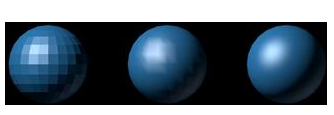
\includegraphics[width=0.3\textwidth]{shading.png}
        \caption{Illusions encountered in Uniform and Gouraud shading.}
    \end{figure}


\end{compactdesc}

\end{multicols}\end{mdframed}





\begin{mdframed}\begin{multicols}{2}
    \begin{figure}[H]
        \centering
        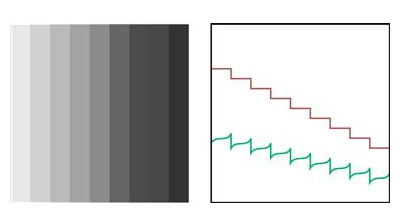
\includegraphics[width=0.3\textwidth]{chevreul_illusion.png}
        \caption{Chevreul illusion, grayscale step patterns}
    \end{figure}
    \begin{figure}[H]
        \centering
        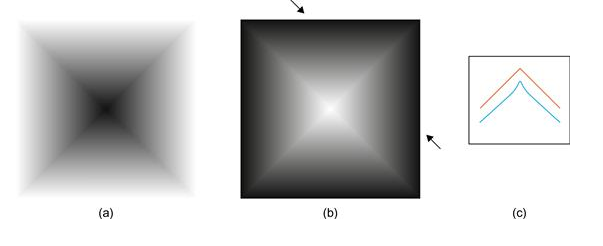
\includegraphics[width=0.3\textwidth]{mach_band_illusion.png}
        \caption{Mach band illusion. Rightmost panel is percevied lightness,
        calculated wiht DoG model.}
    \end{figure}
    \begin{figure}[H]
        \centering
        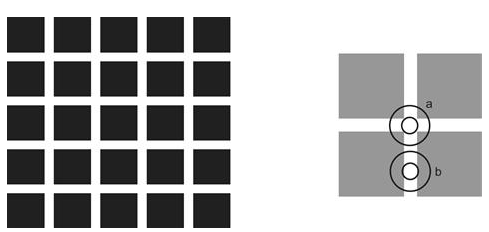
\includegraphics[width=0.3\textwidth]{hermann_grid_illusion.png}
        \caption{Hermann grid illusion. Inhibition may cause the artifacts in
        the grid intersections}
    \end{figure}
    \begin{figure}[H]
        \centering
        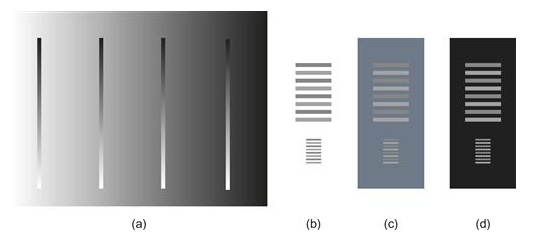
\includegraphics[width=0.3\textwidth]{contrast_crispening.png}
        \caption{Contrast crispening illusion}
    \end{figure}
\end{multicols}\end{mdframed}




\begin{mdframed}\begin{multicols}{2}
\subsection{Luminance, Brightness, Lightness and Gamma}
\begin{compactdesc}
    \item[Constancy] We must know about objects, not light itself. We
        experience colored surfaces, not colored light. Same for the
        overall reflectance of a surface. Black paper looks black under any
        magnitude of light.
    \item[Luminance] measured (real) amount of light
    \item[Brightness] perceived amount of light
    \item[Lightness] perceived reflectance of a surface, its
        gray-scale/saturation.

    \item[V$(\lambda)$ function] relates the sensitivity of the luminance
        channel to wavelength. We are about 100 times more sensitive to
        green light (550nm) than blue (450nm). Red is around 650 nm.
    \item[Finer details] require greater contrast. Minimum 3:1, text should be
        10:1. This limits available colors.
    \item[Brightness] perceived brightness (of a self-luminous source) is
        nonlinear related to the amount of light emitted by a lamp.
    \item[Sensation] $= aI^n$, intensity I. Also applies to other sensations:
        heaviness, smell, touch.
    \item[Monitor gamma] pixels emit nonlinear, gamma around 2.0 cancels a
        brightness power $n = 0.5$ to produce linear perceived brightness.
    \item[Lightness constancy] Help factor out the effects of amount and color
        of light. 1.\@ adaptation to available light. 2\@ lateral inhibition.
    \item[Huge range] amount of light in a dimly lit room is 10,000 times
        darker than that available on a bright day. \textbf{Photopigment} is
        bleached at high light levels, regenerates at lower levels.
    \item[Simultaneous contrast effect] can help us distinguish white from gray
        even though the two surfaces are on backgrounds of different luminance.
    \item[Contrast on paper and on screen] pictures are not just their image,
        but a surface as well! We perceive the actual gray levels of the
        photographic pigments, as opposed to the gray levels of what is depicted.
        Contrast illusions are stronger on computer displays. They are self
        luminous and there is no fine texture.
\end{compactdesc}
\end{multicols}\end{mdframed}

\begin{mdframed}
\begin{multicols}{2}
    \begin{figure}[H]
        \centering
        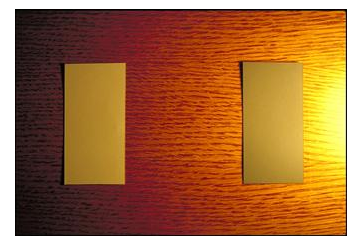
\includegraphics[width=0.7\linewidth]{lightness_constancy.png}
        \caption{Lightness constancy}
    \end{figure}


    \begin{figure}[H]
        \centering
        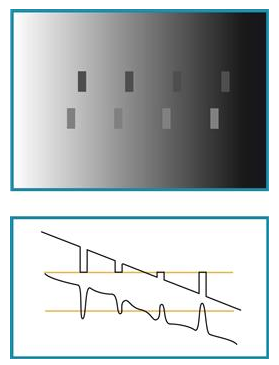
\includegraphics[width=0.4\linewidth]{simultaneous_brightness.png}
        \caption{Simultaneous contrast effect}
    \end{figure}
\end{multicols}\end{mdframed}


\begin{mdframed}
\subsection{Perception of surface lightness}
\begin{multicols}{2}
    The visual system can take into account the fact that a surface turned
    away from the light receives less light.



    We use the lightest object as a \textbf{reference white}.


    \textbf{Glossy highlights} matter. The most important thing separating an isolated
    black-world from a white-world is the ratio between specular and
    non-specular light.
\begin{compactdesc}
    \item[Uniform gray scale] bad, don't use. However, it illustrates some general
        issues related to perceptual scales.
    \item[Weber's law] For small differences in brightness, the value $\delta$
        in $\delta L$ is independent of the overall brightness. Screens
        only have 8 bit luminance, can't show.
    \item[Contrast crispening] Another distortion of gray values. Grays near
        similar gray backgrounds can be differentiated easier (crisper).

\end{compactdesc}
    \begin{figure}[H]
        \centering
        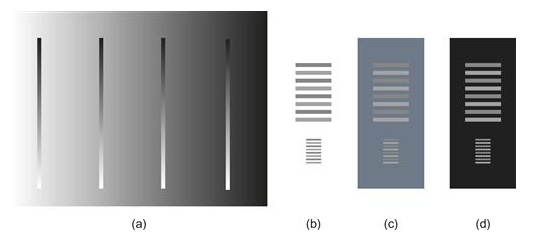
\includegraphics[width=0.3\textwidth]{contrast_crispening.png}
        \caption{Contrast crispening illusion}
    \end{figure}


\end{multicols}\end{mdframed}

\begin{mdframed}
\subsection{Monitor illumination and Monitor surrounds}
Important if accurate color display is needed, like fabric samples on
customer's screen, or for an artist's screen. How to setup lightning around
monitor?
\begin{compactdesc}
    \item[Ambient room illumination,] keep screen emission and room ambience
        at similar luminance. (Normal: 5\% to 20\% of screen light is just
        reflected from room). Really bad with white projector screens.
    \item{Contrast reduced} when room light falls on display.
        $L_{monitor} = V^r + A$ where A is ambient illumination, V
        is voltage, L is luminance output for a given gamma.
    \item{Equal voltage steps} \textbf{= equal perceptual steps}, a lower
        gamma is needed. Dark viewing conditions = higher gamma.
    \item{Room} should have a standard light level and illuminant color.
        The white of the monitor should match the white of a paper help up by
        screen.
\end{compactdesc}

\begin{multicols}{2}

\end{multicols}\end{mdframed}
